\tikzstyle{process} = [rectangle, draw, text centered, minimum height=2em]
\tikzstyle{arrow} = [thick,->,>=stealth]
\tikzstyle{connector} = [draw, -latex']

% \node (tikzmaker) [shift={(2.5, -2.25)}] at (7,18.75) {\includegraphics[width=5cm]{áda}};
\begin{tikzpicture}
    \node [draw=none] at (-6, 4) (input-image) {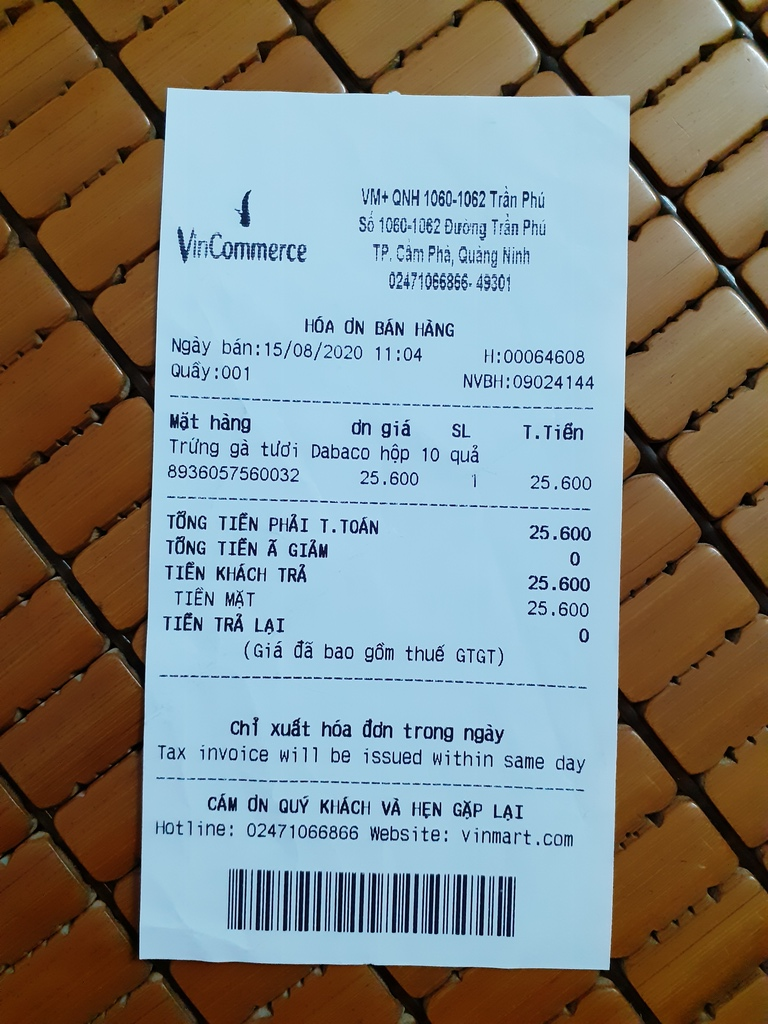
\includegraphics[scale=0.1]{chapter5/images/invoice.png}};
    \node [process] at (0, 0) (text-detection) {
        \begin{tikzpicture}
            \node [process] at (-4, 0) (cnn-fpn) {\footnotesize ResNet50 + FPN};
            \node [process] at (0, 0) (probability) {\footnotesize Probaility Map};
            \node [process] at (0, -1.5) (threshold) {\footnotesize Threshold Map};
            \node [process] at (4, -0.75) (db) {\footnotesize DB post-process};
            \node [draw=none] at (-4, -1.5) (text) {Detection};
            
            \path [connector] (cnn-fpn) -- (probability);
            \path [connector] (cnn-fpn) -- (threshold);
            \path [connector] (probability) -- (db);
            \path [connector] (threshold) -- (db);
        \end{tikzpicture}
    };
    \node [draw=none] at (6, -4) (output-image) {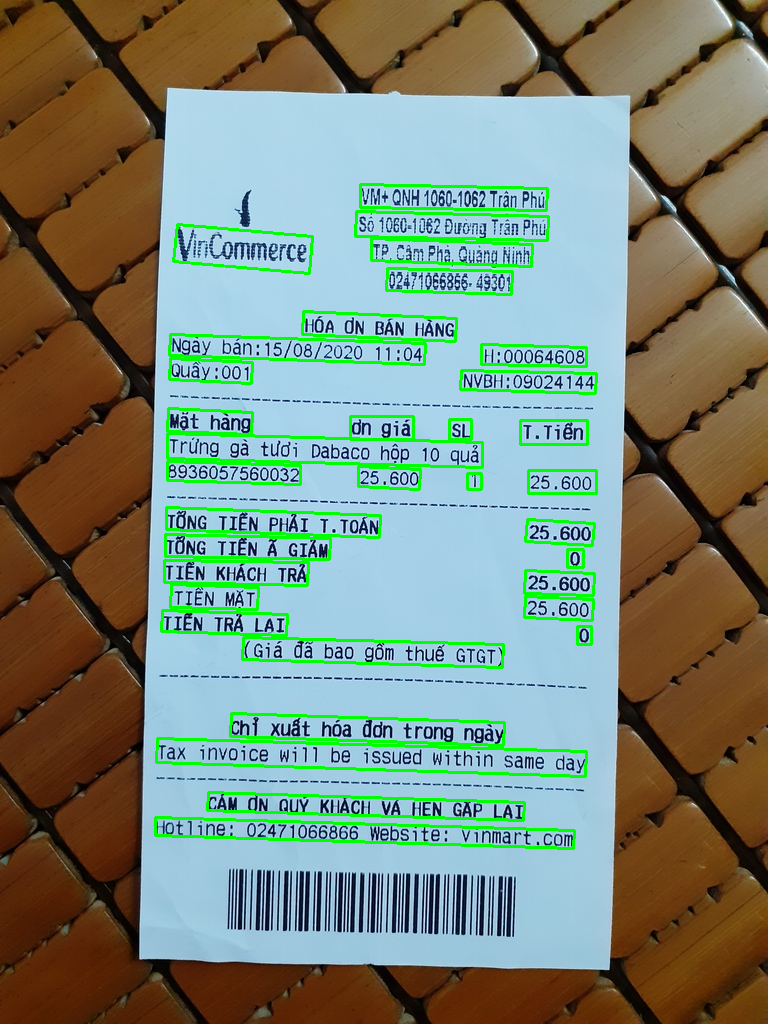
\includegraphics[scale=0.1]{chapter5/images/boudingbox-invoice.png}};

    \draw [arrow] (input-image.south) -- ++ (0, -1) |- (text-detection.west);
    \draw [arrow] (text-detection.east) -- ++ (0, 0) -| (output-image.north);
\end{tikzpicture}